\documentclass[10pt,conference]{IEEEtran}
%\documentclass[letterpaper,twocolumn,10pt]{article}

\usepackage{graphicx}
\usepackage{url}
\usepackage[usenames]{color}
\usepackage{listings}
\usepackage[caption=false]{subfig}


%------------------------------------------------------------------------- 
% take the % away on next line to produce the final camera-ready version 
\pagestyle{empty}

%------------------------------------------------------------------------- 
\begin{document}

\title{Enhancing the security of cloud server configuration with hash chains}


%for single author (just remove % characters)
\author{
{\rm Gautam Kumar, Prof. Brent Lagesse}\\
Computing and Software Systems\\
University of Washington Bothell\\
gautamk@uw.edu, lagesse@uw.edu
} % end author

\maketitle
\thispagestyle{empty}


% At most, 1 page that briefly summarizes your project proposal.  After reading 
% this, a reviewer should understand why you want to do this work, what your 
% general approach is, and what the benefits will be when you complete the work.
\section{Executive Summary}
Information security is a difficult problem, especially in cloud computing environments where 
threats to information security are difficulty to identify and mitigate. One such problem is 
managing the sensitive configuration information.

In traditional enterprise deployments developers often stored configuration within code or on config 
files along with code. This was considered a safe practice because the hardware and Operating System 
where code deployment occurred was owned and managed by the enterprise themselves. These systems 
were usually behind a strong firewall so threats were much easier to mitigate. 

In cloud computing environments, where hardware and the underlying software hypervisor are shared 
amoung thousands of customers who could potentially be using the resources of a single data center, 
Threats to security are much more complex and we need a layered strategy to secure our systems. In 
this environment storing sensitive configuration information on disk could potentially be dangerous.


% Detail side channel attacks

One of the ways developers have secured systems in this environment is to use a centralised trusted 
server to store and retrieve sensitive configuration information. The goal of this project is 
investigating ways to improve the security and allow for forward secracy using Hash 
Chains\cite{tian_self-healing_2008}.

\section{Project Description}

% Background

\subsection{Generic cloud architecture}

A simple cloud architecture (figure \ref{fig:generic_cloud_architecture}) generally consists of one 
or more servers respoding to requests from clients\cite{moreno-vozmediano_iaas_2012}. These servers 
are usually behind a load balancer which routes request to each server based on various factors such 
as CPU usage, Memory usage, Request Volume and Response time. These factors also serve as the basis 
for scaling the number of servers. All servers read and write to the central database. 

\subsubsection{Ephemeral nature} To facilitate auto scaling during peak and lean load times all 
servers are expected to be ephemeral. Thus any server can be added or removed from the pool at any 
time. Cloud computing providers are able to achieve such high levels of varied demands by sharing 
the available hardware resources amoung many customers.

\subsubsection{Networking} All cloud providers offer some solution to the problem of networking 
between 
their cloud components. This means that the loadbalancer, servers and the central database will 
appear to be operating on the same local area network. This is achieved through overlay networks or 
some other kind of Software defined network. These networks also tend to be dynamic and ephemeral in 
nature and cloud architects generally have the ability to redefine the network structure.


\begin{figure}
\centering
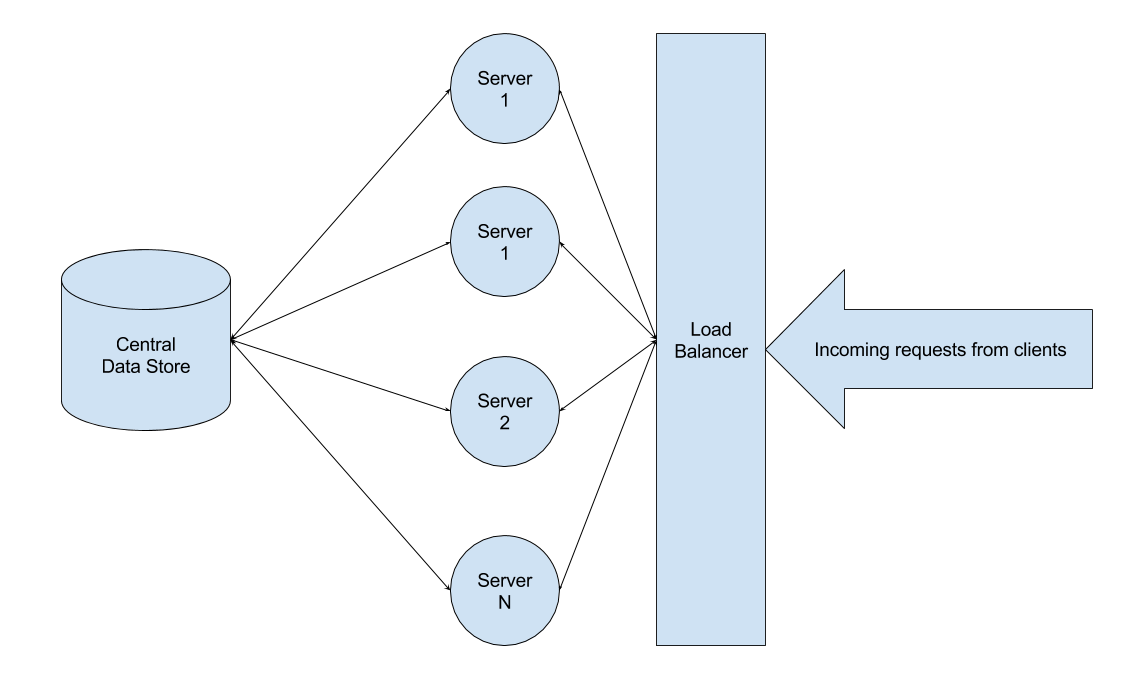
\includegraphics[width=0.7\linewidth]{./generic_cloud_architecture}
\caption[A simple cloud architecture with N servers and a central database]{A simple cloud 
architecture with N servers and a central database}
\label{fig:generic_cloud_architecture}
\end{figure}

\subsection{Sensitive server configuration}
Server configurations can consist of a huge variety of information that is meant to be easily  
modified to change server behaviour. The most valuable and senstive of these are usually database 
credentials and API keys. 

Storing sensitive information such as API Keys and DB credentials along with source code on disk is 
commonly practiced. This practice is highly insecure and should be avoided at all costs because 
of the ease with which data can be recovered from disk in shared 
environments\cite{jordon_cleaning_2012}.

Full disk encryption can help mitigate the risk of data recovery from a shared disk but it 
comes with its own set of pitfalls such as 

\begin{itemize}
\item Information leakage and brute force attacks on disk encryption
\item Side channel attack\cite{ristenpart_hey_2009}
\item Vulnerability in code could lead to a directroy traversal attack\cite{owasp_path_????}
\item Lower server performance requiring more resources leading to higher costs, This can quickly 
add up on large scale cloud deployments with thousands of server instances.
\end{itemize}

Storing configuration as part of code slows down the mitigation effort incase of a breach because 
migrating a large number of servers to the new configuration could take a long time.

\subsection{Centralized Trusted Authority}
A commonly deployed solution to the server configuration problem is using a Centralized Trusted 
Authority (CTA). The concept of trusted authority has existed for a long time \cite{dan_system_2004}.
All servers in a cloud deployment would fetch sensitive configuration information 
from the CTA server during startup and can be easily prompted to reconfigure themselves whenever 
needed there's any change. 

The introduction of a CTA brings with it a new dimension of threats against the whole system such as 

\begin{itemize}
\item CTA Authentication 
\item Client Authentication
\item Client Authorization
\item Attacks against the CTA
\item Trustability of the CTA
\end{itemize}

The aim of the proposed research project is to investigate and propose a method for preventing or 
mitigating one such threat where an attacker has potentially gained command execution access to a 
CTA client. Our research would focus on using hash chains as single use keys to provide 
forwards secrecy\cite{conti_ripp-fs:_2007} and revokability while preventing the attacker from 
gaining access to any sensitive information.

\subsection{Hash Chains}

A hash chain is a set of values obtained by successively hashing a value with a cryptographic Hash 
function. Owing to the one way nature of hash functions, hash chains are directed.

\begin{equation}
x_0 \rightarrow x_1 \rightarrow x_2 \rightarrow x_3 ... x_n
\end{equation}
 where $x_0 = x$, $x_1 = f(x)$ and $x_2 = f(f(x))$. Here $f$ refers to the hashing function. The 
 directed and one way nature of hash chains naturally lends itself to the implementation of single 
 use tokens. 

Single use tokens are key to implementing forward secrecy in this project. Such tokens work well in 
a cloud environment because server instances, as described earlier, are ephemeral. Each server could 
be allocated a hash chain of a certain length and once it runs out the server would no longer be 
able to access sensitive configuration information and would thus be discarded by the load balancer.

\subsection{Activities}

The first step in building a solution to the previously described problem would be to understand the 
attack vectors by constructing a threat model which describes the assumptions and scope of the 
protection mechanism. The next step would be to conduct a feasibility study to investigate the 
potential mechanisms for implementing hash chains as a solution to the problem of forward secrecy. 
The final step would be to build a prototype to demonstrate forward secrecy and re-evaluate the 
threat model describe earlier.

\subsection{Broader Impact}

The system of forward secrecy in stored configurations can be applied to any system operating in a 
potentially untrusted environment where sensitive information needs to be re-deployed / 
re-configured. Some examples include wireless sensor networks, ubiquitous computing devices and IoT 
devices.


\subsection{Related Project}
Confidant\cite{lyft_confidant:_2016} is a project which offers authentication, authorization 
and revokability to clients using a propriatery key management system from amazon.Confidant serves 
as inspiration for our research. Our aim is to build upon some of the concepts implemented in 
confidant and offer revokability and forward secracy without the use of a propriatery Key management 
System.

% Activities

% Survey
% Broader impact
% Why technically rigorous

% The project description must include the activities that you plan for your 
% research.  Provide sufficient background so that a reviewer can understand 
% what you are going to do.  Provide a sufficient survey of related work so that 
% a reviewer understands what work has been done before and where your work will 
% fit in the state of the art (for example, if reputation systems have been 
% built for well-connected networks, but they rely on assumptions that no longer 
% hold in a new type of network, tell the reviewer about the existing state of 
% the art and identify why your new reputation system must be created because 
% the old ones won't work in the new network). You also must include a section 
% on Broader Impacts that describes why your topic is important to the world and 
% a section on Intellectual Merit that describes why the problem you are 
% addressing is technically rigorous.


\bibliographystyle{plain}
\bibliography{CSS539}

\end{document}

